\documentclass[paper=A4,pagesize=auto,12pt,headinclude=true,footinclude=true,BCOR=0mm,DIV=calc]{scrartcl}
\usepackage[english]{babel}
\usepackage[utf8]{inputenc}
\usepackage{graphicx}
\usepackage{geometry}
\usepackage[T1]{fontenc}
\usepackage{lmodern}
\usepackage{amsmath}
\usepackage[scaled]{uarial}
\usepackage{blindtext}
\usepackage{hyperref}
\usepackage{eurosym}
\usepackage{color}
\usepackage{subfigure}
\usepackage{listings}
\usepackage{float}
\usepackage{amsfonts}
\usepackage{amssymb}
\usepackage{graphics}
\usepackage{wrapfig}
\usepackage{setspace}
\usepackage[font=footnotesize]{caption}
\usepackage[format=plain,
justification=RaggedRight,
singlelinecheck=false]
{caption}
\usepackage{textcomp}
\geometry{
	left=2.5cm,
	right=2.5cm,
	top=2.5cm,
	bottom=2cm,
}
\makeatletter
\newcommand{\MSonehalfspacing}{%
	\setstretch{1.44}%  default
	\ifcase \@ptsize \relax % 10pt
	\setstretch {1.44}%
	\or % 11pt
	\setstretch {1.44}%
	\or % 12pt
	\setstretch {1.44}%
	\fi
}
\MSonehalfspacing
\setlength{\parindent}{0pt}

\begin{document}
	
	\title{Smart Pathing\\
	\small{Ausarbeitung im Zuge des Praktikums Parallele Programmierung}}
	\author{\textbf{Rami Aly, Christoph Hueter}\\
	\\University of Hamburg}

	\maketitle
	
	\newpage
	
	\section{Abstract}
	In dieser Arbeit wird die parallelisierte intelligente Wegfindung und Bewegung von Objekten durch einen Graphen für den Anwendungsbereich des Hochleistungsrechnen simuliert.\\
	
	Hierfür wurde das Programm in zwei Teile unterteilt. Im ersten Abschnitt wird eine Routingtable erzeugt, eine Tabelle in der für selektierte Knoten der optimale Pfad und dazugehörige Eigenschaften zu allen Anderen ausgewählten Knoten gespeichert wird. Zwei implementierte Parallelisierungsstrategien werden miteinander verglichen und Verwendungszwecke erörtert.
	
	Abschließend wird die parallelisierte Bewegung der Objekte im Graphen simuliert. Der Pfad des Objektes wird in Abhängigkeit der Pfade aller weiteren Autos gewählt. Ziel hierbei ist es, alternative Pfade zu erkennen, auf denen ein Auto sein Ziel trotz längerer Strecke schneller erreichen kann.
	
	
	\newpage
	
	\tableofcontents 
	
	\newpage
	\section{Kontext}
	Mit der zunehmenden Kostenreduzierung und Verwendung einfacher Kleincomputer in alltäglichen Gegenständen eröffnen sich viele Möglichkeiten in unterschiedlichsten Bereichen der Fortbewegung. Bekannt unter dem Namen Internet of Things ermöglicht dies vielfältige und ausgeprägte Kommunikation zwischen Fahrzeugen und Akteueren auf den öffentlichen Straßen. In Kombination mit der momentanen Entwicklung des autonomen Fahrens eröffnen sich neue Möglichkeiten und Verbesserung im Bereich der optimalen Wegfindung im Straßenverkehr.
	
	Durch kontinuierliche Kommunikation zwischen Autofahrern über eine lange Distanz lassen sich mögliche Ballungsräume vorhersehen und klug durch Umlenkung der Route umgehen oder schwächen, sodass die Ziele der Marken schneller erreicht werden, als beim standardmäßigen Wählen des kürzesten Pfades
	Die Folge wäre ein deutlich effizienterer Straßenverkehr, in denen die Zeit zum Erreichen des Ziels im Durchschnitt minimiert werden kann. Aufgrund der hohen Komplexität und gute Skalierbarkeit vieler Straßennetze eignet sich dieses Problem mit bestimmten Einschränkungen (im Folgenden erläutert) als Berechnungsaufgabe, die durch einen Hochleistungsrechner übernommen werden kann.
	
	\section{Problem- und Modellbeschreibung}
	Da dieses Problem in ihrer Ausführlichkeit äußerst komplex ist schränken, wir das Problem auf ein berechenbares und zugleich gut parallelisierbares Problem ein. 
	Hierfür wird ein gerichteter Graph $G = (V,E)$ mit Kantengewichtsfunktion $f$ betrachtet. Jede Kante hat des weiteren eine Kapazität c, die die maximale Anzahl an Marken beschreibt, die sich auf ihre befinden können. Marken bewegen sich durch Kanten, benötigen also eine Zeit $\Delta t$ bis die Marke die Kante verlassen kann. Knoten aus $S \subseteq V$, fortgehend als Spawner bezeichnet, stellen Eintrittspunkte der Marken in den Graphen dar. Jeder Knoten $v \in V \setminus S$ beherbergt die Funktionalität einer Ampel und regelt den Übergang von Marken zwischen zwei Kanten.
	
	In diesem Modell ist also das Ziel eine Simulation zu erzeugen, in der die Marken durch Bekanntgabe der Pfade und Zeiten der weiteren Marken Ballungsräume und Staus verhindert werden können.
	
	\section{Sequentielles Programm}
	
	\subsection{Lösungsansatz}
	Unsere Lösung kann grundlegend in zwei Teile eingeteilt werden.
	
	Die erste große Aufgabe besteht darin, die kürzesten Pfade zu ermitteln. Wir verwenden das Konzept der Routing-Tabellen, hauptsächlich bekannt für die Kommunikation in einem Netzwerk \cite{RoutingTabelleNetzwerk}. Es wird paarweise die kürzeste Distanz zwischen den Knoten in $S$ bestimmt und in einer Tabelle abgespeichert. Daneben werden für jeden Pfad die Kosten $c[x,y]$ und somit auch sehr einfach die nächstgelegenen k Nachbarn $Q_{k}(n)$ für alle Knoten in $S$ bestimmt.
	Betritt nun eine Marke mit Zielknoten $w$ den Graphen an Knoten $v$, so kann der konventionell kürzeste Pfad aus der Routingtabelle RB[w,v] abgelesen werden. Im folgenden werden insbesondere auch die Kantengewichte der jeweiligen Kanten $e$ zu dem approximierten Zeitpunkt $t_{e}$ in dem eine Marke die Kante $e$ erreicht, abgelesen werden. Je mehr Marken eine Kante passieren möchten, desto höher ist das Kantengewicht. Die Gesamtkosten, den Pfad zu wählen ergeben sich aus beiden Faktoren, sowie die Distanz (Luftlinie) vom ursprünglichen Ziel $w_{m}$ und :\\
	
	\begin{equation}
	\theta(v,w)  = c[v,w] + \sum_{e \in RT[v,w].E} f_{e}(t_{e}) + dist(w_{m}, w)
	\end{equation}

	Sollte ein alternativer Pfad $(v,w')$ gewählt werden, so muss bei gleicher Entfernung zu $v$ gelten :
	
	 $\sum_{e \in RT[v,w'].E} f_{e}(t_{e}) < \sum_{e \in RT[v,w].E} f_{e}(t_{e}) + dist(w_{m}, w')$\\
	 
	Im Fall, dass $k$ > 2 sein könnte, also mehr als 1 Nachbar betrachtet wird, sucht man den Pfad mit minimalen Kosten:\\
	
	\begin{equation} 
	\theta_{min}(v,w) = min(\theta(v,w) | w \in Q_{k}(v))
	\end{equation}

	Nach der Auswahl des besten Pfades für die Marke werden die Kantengewichte aktualisiert. Jede Kante verfügt über eine Timetable. In ihr wird für jeden Step der Simulation ein Kantengewicht abgespeichert. Dies dient dazu, zu wissen, wann Marken die Kante vermutlich werden. 
	
	Die Auswahl des Index der Timetable in dem der Wert nach dem Auswählen der Route erhöht werden soll wird über eine Heuristik bestimmt: $\frac{2* c[v,w]}{TL_Count}$. Es wird also ein kleiner Index in der Timetable gewählt, sollten viele Ampeln auf dem Weg liegen.
	
	Verlässt eine Marke eine Kante, so wird der Wert in der Timetable aktualisiert. 
	
	Des Weiteren muss die Bewegung der Marken im Graph simuliert werden.
	
	CHRISTOPH
	CHRISTOPH...Paar Gedankenanstöße: Des Weiteren befinden sich die Marken in eine Warteschlange, in der zusätzlich die Distanz bis zum Ende der Kante gespeichert wird. Alle Marken bewegen sich mit der gleichen Geschwindigkeit, können sich nicht überholen und haben eine Größe k. 

	 
	 
	 \subsection{Implementierung}
	 Zur Erzeugung des graphens werden Karten aus der Open-Streetmap Datenbank \cite{OSM} verwendet und mittels eines Python-Scripts die Knoten und Kanten extrahiert und in einfachen Textdateien gespeichert. Damit der exportierte Graph optisch der Karte entspricht werden noch zusätzlich die Positionsdaten der Knoten exportiert.
	 
	 Das eigentliche Programm ist in C++ geschrieben. Es werden die Daten des Graphs eingelesen. Als Spawner wurden all jene Knoten ausgewählt. die am Rande des Graphens liegen, also lediglich mit 2 Kanten verbunden ist. Natürlich lassen sich Spawner auch anders auswählen. Interpretieren könnte man dies, dass lediglcih der Rand des Graphens eine Auffahr/Abfahrt einer Karte, beispielsweise Autobahn darstellt.
	 
	 Zur Berechnung der Pfade für die Routingtable wird die Boost Graph Library(BGL) \cite{Boost} verwendet und in Version 1.61 bis 1.65.0 getestet. Es wird der A*-Algorithmus verwendet und als Heuristik die klassische Methode der Luftlinie verwendet. Des Weiteren haben wir mehrere Optimierungen aufgrund vorhandener Redundanz eingebaut. Beispielsweise ist der optimale Pfad von v zu w der Gleiche wie von w zu v und wird aus diesem Grund nicht doppelt berechnet. 
	 Die TimeTable sollte so groß sein, dass das Auto welches in der Theorie den spätesten Eintrag in einer Table setzen kann, nicht größer als die Tabelle selbst ist, da sonst Einträge um eine gesamte Iteration der Timetable zu früh gesetzt werden. 
	 
	 CHRISTOPH, schreib hier was zu der implementierung der beweung der Autos hin. und Trafficlight, Knoten etc.....gibs ja viel zu erzählen
	
	
	\newpage
	
	\section{Parallelisierung}
	Während das Preprocessing und die Visualisierung weiterhin sequenziell durchlaufen werden, sind Berechnung und Erzeugung der Routingtabelle, sowie Simulation von uns parallelisiert worden. Hierfür wurde MPI verwendet, also das Parallelisierungsverfahren des message passing.
	\subsection{RoutingTable}
	Zur Berechnung der Routingtabelle haben wir zwei verschiedene Parallelisierungsstrategien implementiert, da beide über ihre anwendungsbezogenen Vor- und Nachteile verfügen.
	\subsubsection{Berechnung sequenziell, parallelisiert}
	Bei dem ersten Verfahren (Methode A) kennt jeder Prozess die gesamte Karte. Zu Beginn werden die Spawner möglichst gleichmäßig auf alle Prozesse zugewiesen. Jeder Prozess berechnet dann für die zugewiesenen Spawner die Routingtabelle zu allen anderen Spawner des gesamten Graphen. Sind beispielsweise u, v ,y Spawner, und $p_{1}$ sowie $p_{2}$ Prozesse, dann könnte u und v $p_{1}$ zugewiesen werden. Nun berechnet  $p_{1}$ die Routingtabelle mit den Pfaden zwischen uu,uv,uy,vv....
	Für das Verteilen der Spawner auf die Prozesse wurde MPI\_Scatterv verwendet.
	
	Nachdem jeder Prozess mit der Berechnung der Routingtabelle abgeschlossen ist, sammelt jeder die Routingtabellen der anderen Prozesse. Dafür müssen die Routingtabelle in eine für MPI sinnvolle Struktur konvertiert werden. Hierfür wird die Routingtablle in eine Zweidimensionalen Array umgeformt, die kontinuierlich im Speicher abgelegt ist. Dadurch kann ohne Weiteres der Pointer zu dem Array weitergegeben werden. Das sammeln geschieht mit MPI\_Gatherv, und wird von allen Prozessen ausgeführt, da im Anschluss alle Prozesse die komplette Rourtingtabelle erhalten sollen.\\
	Da auch die Kosten parallelisiert berechnet werden, werden diese im nächsten Schritt auf dem gleichen Wege zu allen anderen Prozessen kommuniziert. 
	
	
	Wir haben uns dazu entschieden, die Berechnung der nächsten Nachbarn nicht parallelisiert auszuführen, da ein Großteil der Informationen bereits durch die Kosten versendet wurde und der Rechenaufwand ausgenommen von äußerst großen Karten kleiner ist als der Overhead durch die Kommunikation.
	
	\label{parallelA}
		\begin{figure}[H]
			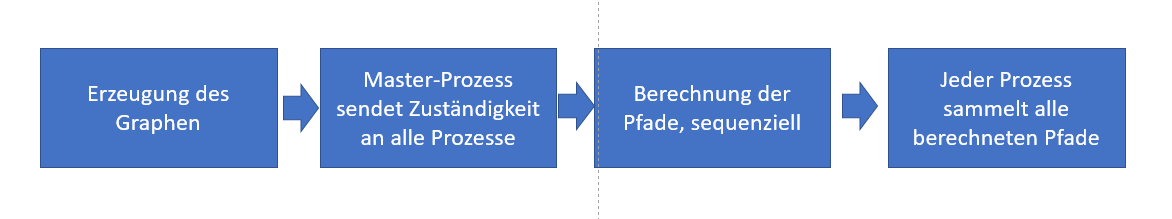
\includegraphics[scale = 0.80]{Prasentation/AblaufParallelA.png}
			\caption{Konzept der Scatterv/Gatherv Parallelisierung}
		\end{figure}
	
	\subsubsection{Berechnung parallel, nacheinander}
	Bei der alternativen Parallelisierungsmethode (Methode B) wird der Graph auf die Prozesse aufgeteilt \ref{boostGraph} und die Berechnung des optimalen Pfades parallelisiert durchgeführt und dies für alle Paare von S nacheinander ausgeführt. Es wird also der Algorithmus selbst parallelisiert, während das Programm selbst sequenziell läuft. Zur Implementierung haben wir auf die Parallel BGL zurückgegriffen [\cite{ParallelBGL}. Die Library verwendet zur Kommunikation Boost::MPI. Da ein parallelisierter A* nicht in der Library vorhanden war, haben wir auf den Dijkstra-Algorithmus zurückgegriffen.
	
	Zu Beginn wird der Graph auf alle Prozesse möglichst gleichmäßig aufgeteilt \ und alle Eigenschaften die in dem Graph gespeichert werden sollen, definiert. In unserem Falle ist der Vorgänger eines Knotens $v \in V$ eine solche Eigenschaft, die von dem Dijkstra-Algorithmus gesetzt wird.
	Hierbei handelt es sich um eine verteilte Property-Map, das heißt, dass der vom Algorithmus gefundene beste Vorgänger p[v] grundsätzlich nur im Prozess gespeichert ist, dem der Knoten gehört (manchmal existieren Vorgänger die lediglich als Platzhalter dienen \ref{boostProp}). Existiert also eine Kante von einem Knoten v in  $p_{1}$ zu einem Knoten außerhalb, so muss eine Anfrage an den anderen Prozess gestellt werden, die Information über den außenstehenden Knoten zu erhalten.
	
	Damit jeder Prozess nach Abschluss der Berechnungen auch die gesamte Routingtabelle zur Verfügung stehen hat, muss eine Anfrage (request) gestellt werden, dass der Besitzer eines fremden Knoten den Vorgänger übersenden soll. ist dies für alle fremden Knoten getan ist die Routingtabelle für alle Prozesse vollständig.
	
	\label{boost}
	\begin{figure}[H]
		\subfigure{\label{boostGraph}\includegraphics[scale = 0.80]{Prasentation/distributed-Graph.png}}
		\subfigure{\label{boostProp}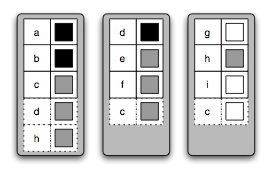
\includegraphics[scale = 0.80]{Prasentation/dist-pmap.png}}
		\caption{Konzept Parallel BGL}
		\cite{ParallelBGLPicture}
	\end{figure}
	
	
	\subsection{Simulation}
		
		Christoph
	
	\section{Leistungsanalyse und Skalierbarkeit}
	Zur Messung der Laufzeit wurden Hauptsächlich aus einem Graphen mit 424 Knoten und Kanten 1244. Es wurden zur Berechnung 1 Knoten reserviert.
	
	Die Messergebnisse entsprechen dem Durchschnitt aus 5 Messungen.
	\subsection{RoutingTable}
	\subsubsection{Methode A}
	Oprofile wurde zu Beginn für das sequenzielle Programm verwendet. Neben einigen Memoryleaks ist uns da jedoch nichts negativ aufgefallen. Zur Performanceanalyse wurde hauptsächlich Vampir verwendet.  Man erkennt sehr deutlich die Phasen in denen MPI\_Kommunikation stattfindet. Die Phase zwischen dem MPI\_Init und MPI\_vScatter wird für die Erzeugung des Graphens benötigt. Unserer Meinung nach ist das Verhältnis zwischen Komunikation und Performance angemessen. Vergleicht man die Kommunikation zwischen 8 und 16 Prozessen, so ist beim Scatter ein deutlicher Kommunikationszuwachs erkennbar \ref{vampirA}. Erstaunlicher Weise ist trotz dem vGather, der von allen Prozessen ausgeführt wird, der Overhead recht gering.\\
	\label{vampirA}
	\begin{figure}[H]
		\includegraphics[scale = 0.40]{Prasentation/vampirmethodA.png}
		\caption{Vampir Visualisierung 8 und 16 Prozesse}
	\end{figure}
		
	Negativ aufgefallen ist uns die doch vergleichsweise lange Zeit die benötigt wird, um den Graphen zu erzeugen. Nach Amdahls Gesetz \cite{PaPoBuch} ist beim Strong Scaling Speedup des gesamten Programmes limitiert durch den sequenziellen Anteil des Programmes, sodass die Effizienz bei niedrigerem Parallelisierungsanteil deutlich geringer ausfällt. Mit einem maximalen Speedup von 5.8 sind die Ergebnisse bei 15 (Efizienz: 0.39) insgesamt jedoch zufriedenstellend.
		\label{speedUpA}
		\begin{figure}[H]
			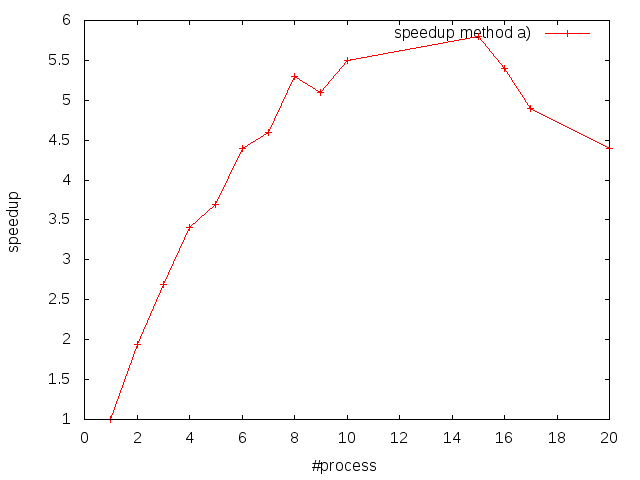
\includegraphics[scale = 0.55]{Prasentation/speedupPa.png}
			\caption{Vampir Visualisierung 8 und 16 Prozesse}
		\end{figure}
	
	\subsubsection{Methode B}
	Bei der Analyse mit Vampir ist sehr schnell aufgefallen, dass die Anzahl der Kommunikation für 2 Prozesse recht groß und ist. Der Overhead erhöht sich dramatisch bei 8 Prozessen.
		\label{vampirB}
		\begin{figure}[H]
			\includegraphics[scale = 0.38]{Prasentation/vampirmethodB.png}
			\caption{Vampir Visualisierung 8 und 16 Prozesse}
		\end{figure}
	Demzufolge sieht die Skalierbarkeit bei dem fest gewählten Problem sehr negativ aus. Es wird sogar deutlich länger gebraucht, als für das sequenzielle Programm, da der Mehrwert der Parallelisierten Berechnung wohl nicht im geringsten den Kommunikations-overhead rechtfertigt:
	\label{speedUpB}
	\begin{figure}[H]
		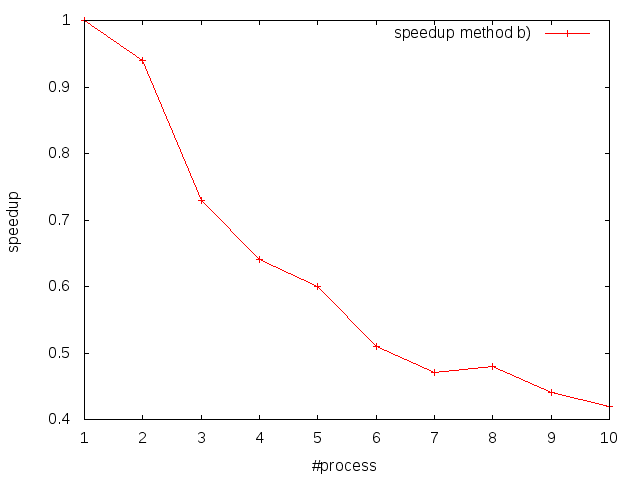
\includegraphics[scale = 0.55]{Prasentation/speedupPBoost.png}
		\caption{Speedup Methode A}
	\end{figure}
	Zu Beginn waren wir darüber recht verwundert, haben uns genauer die von Boost dargestellten Ergebnisse analysiert und gemerkt, dass erwarteter Weise die Dimension des Graphens um ein Vielfaches größer ist. Getestet wurde mit 1 Millionen Knoten und 15 Millionen Kanten\cite{DijkstraBoost}. Anscheinend lohnt es sich erst ab unglaublich großen Graphen die Wegfindung mit dem parallelen Dijksta zu gestalten. Abschließend haben wir einen Graphen mit 16700 Knoten und 39982 Kanten getestet und sind bei 2 Prozessen inzwischen bei einem 'Speedup' von 0.976 anheben, was eine Verbesserung darstellt \ref{speedUpB}.
	
	Übersehen sollte man jedoch auch nicht, dass sich Gustafsons Gesetz \cite{PaPoBuch}, also bezüglich des Weak Scalings nicht ohne Weiteres auf unsere Simulation übertragen lässt, da bei einer Vergrößerung der Dimension des Problemes der sequenzielle Teil ebenfalls deutlich komplexer wird, und eine Aussage über das Verhältnis zwischen parallelem und sequenziellen Programm bei komplexer werdendem Problem zusätzlich herausgefunden werden müsste.
	\subsubsection{Vergleich}
	Es werden bei beiden Methoden unterschiedliche Probleme in Teilaufgaben zerlegt. Bei Methode A wird das Berechnen der Einträge der Routingtabelle parallelisiert, während in Methode B das Berechnen des kürzesten Pfades parallelisiert wird. Dies wirkt sich signifikant auf die Granularität der Verfahren aus.
	
	Es sollte recht eindeutig aus den Ergebnissen folgen, dass für kleinere Graphen die Methode A deutlich bessere Ergebnisse hinsichtlich der Skalierbarkeit erziehlt. Die Granularität ist bei dieser Methodik nicht zu fein. Beobachtbar war jedoch auch, dass bei einer linearen Vergrößerung der Anzahl der Prozesse der Overhead des Scatterv stärker als linear zunimmt und möglicherweise bei sehr großen Graphen, also wenn das betrachtete Problem vergrößert wird, zur ausreichend schnellen Lösung eine Anzahl von Prozessen benötigt wird, die den Overhead relevant werden lassen.
	
	Hier sehen wir den eigentlich einzigen Anwendungsbereich der Methode B). Diese Vorgehensweise beginnt sich erst bei unglaublich großen Graphen zu lohnen und bringt dann eine akzpetable Skalierbarkeit bei gleichbleibendem Problem mit sich \ref{speedUpB}. Bei dem von uns durchgeführten Graphen ist die Granularität in Anbetracht des Overheads zu fein. Es muss deutlich weniger gerechnet werden, als ausgetauscht.\\
	Die Kombination beider Verfahren könnte beispielsweise dahingehend genutzt werden, dass für äußert komplexe Graphen Methode A das Problem der Berechnungen zerteilt und auf jede dieser Teile dann die Methode B) verwendet wird.

	
	
	
	
	
	
	Während bei dem Sequenziellen Durchlauf 3.5 Sekunden benötigt werden, wird bei 15 Prozessen ein Minimum von 0.604 Sekunden erreicht.
	\section{Verbesserungen und Ausblick}
	An vielen verschiedenen Stellen lassen sich noch mögliche Ausbaumöglichkeiten finden. Die Approximation zum bestimmen des Indexes in der Timetable könnte dahingehend optimiert werden, dass genau berechnet wird, welche Ampeln grün sein werden, wenn das Auto dort ankommt und von welchem Typ die Ampel (Kreuzung, T-Straße...). 
	
	
	Darüber hinaus ist der parallelisierte Dijkstra zur Berechnung der Routingtabelle nicht der schnellste parallele Wegfindungsalgorithmus, der von der Parallel BGL zur Verfügung gestellt wird. Hier könnte man überlegen, beispielsweise den Eager Dijkstra Algortihmus oder den Delta-Stepping shortest path Algorithmus zu verwenden, die besseren strong scaling haben.
	
	
	Hinzu kommt die Möglichkeit statt eines Gatherv für alle Prozesse ein Alltoallv zu verwenden, um möglichen Overhead zu reduzieren.
	
	Ein weiterer relevanter Aspekt wäre das Aktuallisieren der Werte in den Timetables, nachdem eine Marke gespawned wurde. Bei großer Distanz wird die Heurisik ungenau, auch wenn man sie wie oben vorgeschlagen verbessern sollte. Die Überlegung besteht, den hinzuaddierten Wert bei größerer Distanz zu reduzieren, beispielsweise um $\frac{1}{distance}$.
	
	Des Weiteren besteht natürlich die Möglichkeit Teile des Programmes mit OpenMP zu parallelisieren, die über Shared Memory verfügen. MPI würde also nur zur Kommunikation zwischen Prozessen verwendet werden, die nicht über einen gemeinsamen Speicher verfügen.
	
	\section{Removing irrelevant information from selected features}
	
	
	
	\newpage
	
	\begin{thebibliography}{xxxxxx}
		\bibitem [1] {RoutingTabelleNetzwerk}Wikipedia, Routing table  (17.09.2017) \url{https://en.wikipedia.org/wiki/Routing_table}
		\bibitem [2] {OSM} OpenStreetMap \url{https://www.openstreetmap.de/}
		\bibitem [3] {Boost} Boost c++ Libraries: \url{http://www.boost.org/}
		\bibitem [4] {ParallelBGL} Parallel Boost Graph Libary \url{http://www.osl.iu.edu/research/pbgl/}
		\bibitem [5] {ParallelBGLPicture} Parallel Boost Graph Library Overview \url{http://www.boost.org/doc/libs/1_65_1/libs/graph_parallel/doc/html/overview.html}
		\bibitem[6]	 {PaPoBuch} Zbigniew J. Czech (2016): 'Introduction to Parallel Computing', S. 69f.
		\bibitem[7] {DijkstraBoost} Dijkstra shortest paths, Parallel BGL \url{http://www.boost.org/doc/libs/1_65_1/libs/graph_parallel/doc/html/dijkstra_shortest_paths.html}
	\end{thebibliography}
	

	
	
\end{document}



